\documentclass[aspectratio=169, 10pt]{beamer}

% ─── Theme ────────────────────────────────────────────────────────────────────
\usetheme[progressbar=frametitle, sectionpage=progressbar, block=fill]{metropolis}

% ─── Colour palette ───────────────────────────────────────────────────────────
\definecolor{sotonblue}{HTML}{003B5C}
\definecolor{sotongold}{HTML}{C4A000}
\definecolor{sotongrey}{HTML}{F5F5F5}

\setbeamercolor{palette primary}{bg=sotonblue}
\setbeamercolor{frametitle}{bg=sotonblue, fg=white}
\setbeamercolor{progress bar}{fg=sotongold, bg=sotonblue!30}
\setbeamercolor{alerted text}{fg=sotonblue}
\setbeamercolor{block title alerted}{bg=sotonblue, fg=white}
\setbeamercolor{block body alerted}{bg=sotonblue!8}
\setbeamercolor{block title}{bg=sotongold!80!black, fg=white}
\setbeamercolor{block body}{bg=sotongold!10}

% ─── Packages ─────────────────────────────────────────────────────────────────
\usepackage{booktabs}
\usepackage{tikz}
\usetikzlibrary{shapes.geometric, arrows.meta, positioning, calc, backgrounds}
\usepackage{graphicx}
\usepackage{xcolor}
\usepackage{amsmath}
\usepackage{array}
\usepackage{colortbl}
\usepackage[T1]{fontenc}
\usepackage{microtype}

% ─── Metadata ─────────────────────────────────────────────────────────────────
\title{Introduction to Machine Learning}
\subtitle{Southampton Statistics Summer School}
\author{Brody Hannan}
\institute{University of Southampton}
\date{30 July 2026}

% ─── TikZ styles ──────────────────────────────────────────────────────────────
\tikzset{
  flowbox/.style={
    draw=sotonblue, fill=sotonblue!10, rectangle, rounded corners=4pt,
    minimum width=2.0cm, minimum height=0.85cm, align=center,
    text width=1.9cm, font=\scriptsize
  },
  flowarrow/.style={-Stealth, thick, color=sotonblue},
  treeq/.style={
    draw=sotonblue, fill=sotonblue!10, rounded corners=4pt,
    minimum width=2.5cm, minimum height=0.65cm,
    align=center, text width=2.3cm, font=\scriptsize
  },
  treeleaf_y/.style={
    draw=green!60!black, fill=green!15, rounded corners=3pt,
    minimum width=1.6cm, minimum height=0.55cm,
    align=center, font=\scriptsize\bfseries
  },
  treeleaf_n/.style={
    draw=red!60!black, fill=red!12, rounded corners=3pt,
    minimum width=1.6cm, minimum height=0.55cm,
    align=center, font=\scriptsize\bfseries
  }
}

% ─────────────────────────────────────────────────────────────────────────────
\begin{document}

\maketitle

% ─── SCOPE ───────────────────────────────────────────────────────────────────
\begin{frame}{Today's Workshop}
\begin{columns}[T]
\begin{column}{0.48\textwidth}
\textbf{Part 1: Theory} \hfill \textcolor{sotongold}{\textit{45 min}}
\begin{itemize}
  \setlength\itemsep{0.4em}
  \item Why ML for social science?
  \item What ML is and what it is not
  \item The ML workflow
  \item Supervised vs.\ unsupervised learning
  \item Decision trees
  \item Random forests
  \item Gradient boosting
  \item Model evaluation
  \item Ethical limits
\end{itemize}
\end{column}

\begin{column}{0.48\textwidth}
\textbf{Part 2: Practical} \hfill \textcolor{sotongold}{\textit{75 min}}
\begin{itemize}
  \setlength\itemsep{0.4em}
  \item Google Colab notebook (Python)
  \item 1994 US Census income data
  \item Build and compare three models
  \item Interpret variable importance
  \item Reflection questions throughout
  \item Extension: clustering
\end{itemize}

\vspace{1.2em}
\small
\textbf{All materials:}\\
\texttt{github.com/BHannan01/}\\
\texttt{introduction-to-machine-learning}
\end{column}
\end{columns}
\end{frame}

% =============================================================================
\section{Why Machine Learning?}

\begin{frame}{Activity: Who Earns More Than \$50K?}

\begin{center}
\small
\renewcommand{\arraystretch}{1.35}
\begin{tabular}{lllll}
\toprule
\textbf{Person} & \textbf{Age} & \textbf{Education} & \textbf{Occupation} & \textbf{Hrs/week} \\
\midrule
Alex   & 28 & High school    & Service worker   & 35 \\
Jordan & 45 & Bachelor's     & Manager          & 55 \\
Sam    & 32 & Master's       & Tech worker      & 40 \\
Casey  & 52 & No diploma     & Farming          & 45 \\
Morgan & 38 & Bachelor's     & Self-employed    & 60 \\
\bottomrule
\end{tabular}
\end{center}

\vspace{0.5em}
\textbf{Take 60 seconds. Rank these five people from most to least likely to earn $>$\$50K per year.}

\vspace{0.6em}
\begin{columns}[T]
\begin{column}{0.48\textwidth}
\textbf{Then ask yourself:}
\begin{itemize}
  \setlength\itemsep{0.3em}
  \item What information did you use?
  \item What information would have made you more confident?
  \item Can you write down the exact rule you applied?
\end{itemize}
\end{column}
\begin{column}{0.48\textwidth}
\begin{alertblock}{This is exactly what ML does}
A machine learning model learns those rules automatically from data -- for 48,842 real people at once -- and tells you which rules it used.
\end{alertblock}
\end{column}
\end{columns}
\end{frame}

\begin{frame}{What This Enables at Scale}
\begin{columns}[T]
\begin{column}{0.57\textwidth}
\textbf{Mapping Social Mobility (Chetty et al., 2018)}
\begin{itemize}
  \setlength\itemsep{0.35em}
  \item ML applied to US tax records covering 20 million families
  \item Identified neighbourhood-level predictors of upward mobility across 742 commuting zones
  \item Key finding: social capital, school quality, and commute times predicted adult income better than individual-level variables alone
  \item Produced a policy-relevant map of opportunity that traditional regression alone could not have generated at this scale
\end{itemize}
\end{column}
\begin{column}{0.40\textwidth}
\begin{alertblock}{The point}
Your intuitive ranking of five people is slow, inconsistent, and hard to audit. ML makes the process systematic, scalable, and transparent -- but introduces its own risks.
\end{alertblock}
\vspace{0.5em}
\small\textit{Chetty, R., et al.\ (2018). The opportunity atlas. NBER Working Paper 25147.}
\end{column}
\end{columns}
\end{frame}

% =============================================================================
\section{What Is Machine Learning?}

\begin{frame}{"AI" is Not the Same as Machine Learning}
\begin{columns}[T]
\begin{column}{0.46\textwidth}
\vspace{0.3em}
\resizebox{\linewidth}{!}{%
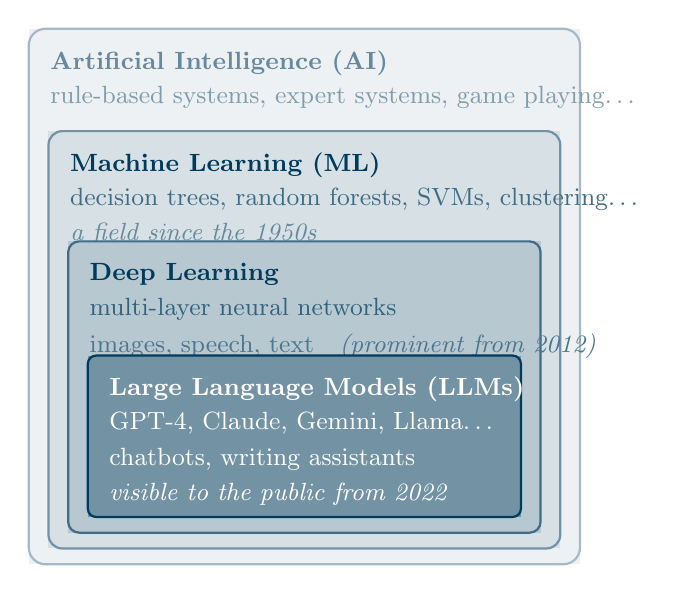
\begin{tikzpicture}[font=\small]
% AI (outermost)
\fill[sotonblue!7]  (0,0) rectangle (7.0, 6.8);
\draw[sotonblue!35, rounded corners=6pt, thick] (0,0) rectangle (7.0, 6.8);
\node[sotonblue!60, anchor=north west, font=\small\bfseries] at (0.15,6.65) {Artificial Intelligence (AI)};
\node[sotonblue!50, anchor=north west, font=\small] at (0.15,6.20) {rule-based systems, expert systems, game playing\ldots};

% ML
\fill[sotonblue!16] (0.25,0.2) rectangle (6.75,5.5);
\draw[sotonblue!55, rounded corners=5pt, thick] (0.25,0.2) rectangle (6.75,5.5);
\node[sotonblue, anchor=north west, font=\small\bfseries] at (0.40,5.35) {Machine Learning (ML)};
\node[sotonblue!75, anchor=north west, font=\small] at (0.40,4.90) {decision trees, random forests, SVMs, clustering\ldots};
\node[sotonblue!60, anchor=north west, font=\small] at (0.40,4.45) {\textit{a field since the 1950s}};

% Deep Learning
\fill[sotonblue!28] (0.5,0.4) rectangle (6.5,4.1);
\draw[sotonblue!75, rounded corners=4pt, thick] (0.5,0.4) rectangle (6.5,4.1);
\node[sotonblue, anchor=north west, font=\small\bfseries] at (0.65,3.95) {Deep Learning};
\node[sotonblue!80, anchor=north west, font=\small] at (0.65,3.50) {multi-layer neural networks};
\node[sotonblue!70, anchor=north west, font=\small] at (0.65,3.05) {images, speech, text\quad\textit{(prominent from 2012)}};

% LLMs (innermost)
\fill[sotonblue!55] (0.75,0.6) rectangle (6.25,2.65);
\draw[sotonblue, rounded corners=3pt, thick] (0.75,0.6) rectangle (6.25,2.65);
\node[white, anchor=north west, font=\small\bfseries] at (0.90,2.50) {Large Language Models (LLMs)};
\node[white!85, anchor=north west, font=\small] at (0.90,2.05) {GPT-4, Claude, Gemini, Llama\ldots};
\node[white!75, anchor=north west, font=\small] at (0.90,1.60) {chatbots, writing assistants};
\node[white!65, anchor=north west, font=\small] at (0.90,1.15) {\textit{visible to the public from 2022}};
\end{tikzpicture}}
\end{column}

\begin{column}{0.51\textwidth}
\small
\textbf{NLP} (Natural Language Processing) is an \textit{application domain}, not a method. It uses ML and deep learning to work with human language: translation, sentiment analysis, topic modelling.

\vspace{0.55em}
\textbf{A brief history}
\begin{itemize}
  \setlength\itemsep{0.22em}
  \item \textbf{1950s--70s:} ML emerges within AI research
  \item \textbf{1980s:} ML and AI diverge into separate fields
  \item \textbf{1990s:} ML formalised as its own discipline
  \item \textbf{2010s:} Deep learning revives neural networks at scale
  \item \textbf{2020s:} LLMs make "AI" visible to the public
\end{itemize}

\vspace{0.55em}
\begin{alertblock}{ML is not\ldots}
\begin{itemize}
  \setlength\itemsep{0.18em}
  \item The same thing as AI
  \item Just chatbots -- LLMs are the tip of a large iceberg
  \item New -- the methods we cover today have roots in the 1950s
  \item Always a black box -- decision trees are fully interpretable
\end{itemize}
\end{alertblock}
\end{column}
\end{columns}
\end{frame}

\begin{frame}{ML vs.\ Traditional Statistics}

\begin{center}
\small
\renewcommand{\arraystretch}{1.3}
\begin{tabular}{p{3.2cm} p{4.8cm} p{4.8cm}}
\toprule
 & \textbf{Traditional statistics} & \textbf{Machine learning} \\
\midrule
\textbf{Primary goal}     & Explain relationships          & Predict outcomes accurately \\
\textbf{Starting point}   & Theory and hypothesis          & Patterns in data \\
\textbf{Model form}       & Pre-specified by researcher    & Learned from data \\
\textbf{Output}           & Coefficients, $p$-values, CIs  & Predictions, accuracy, importance \\
\textbf{Core strength}    & Inference and interpretability & Flexibility and performance \\
\textbf{Core limitation}  & Rigid assumptions              & Less directly interpretable \\
\bottomrule
\end{tabular}
\end{center}

\vspace{0.8em}
\begin{center}
\alert{They are complementary tools, not competitors.}\\
\small ML is most useful when prediction is the goal and the data are too complex for a pre-specified model.
\end{center}

\end{frame}

\begin{frame}{The Core Idea: Learning from Labelled Data}

\begin{center}
\resizebox{\textwidth}{!}{%
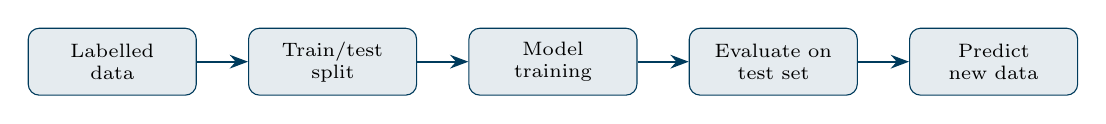
\begin{tikzpicture}
\node[flowbox] (data)   {Labelled\\data};
\node[flowbox, right=0.65cm of data]  (split)  {Train/test\\split};
\node[flowbox, right=0.65cm of split] (train)  {Model\\training};
\node[flowbox, right=0.65cm of train] (eval)   {Evaluate on\\test set};
\node[flowbox, right=0.65cm of eval]  (deploy) {Predict\\new data};

\draw[flowarrow] (data)   -- (split);
\draw[flowarrow] (split)  -- (train);
\draw[flowarrow] (train)  -- (eval);
\draw[flowarrow] (eval)   -- (deploy);
\end{tikzpicture}}
\end{center}

\vspace{0.6em}
\begin{columns}[T]
\begin{column}{0.48\textwidth}
\textbf{Training set (80\%):}\\
The model learns from this data. We use \texttt{stratify=y} to keep the same class proportions as the full dataset.

\vspace{0.5em}
\textbf{Test set (20\%):}\\
Locked away until the very end. Used only to evaluate final performance on cases the model has never seen.
\end{column}
\begin{column}{0.48\textwidth}
\textbf{Why split — and not just train on everything?}\\
A model that memorises training data will look perfect on that data but fail on new cases. The test set gives an honest, unbiased estimate.

\vspace{0.5em}
\textbf{What about class imbalance?}\\
In our dataset, 75\% earn $\leq$\$50K and 25\% earn $>$\$50K. We do \textit{not} balance the classes artificially. \texttt{stratify=y} simply preserves this ratio in both sets.
\end{column}
\end{columns}
\end{frame}

\begin{frame}{Class Imbalance and Why Accuracy Can Mislead}

\begin{columns}[T]
\begin{column}{0.55\textwidth}
\textbf{Our dataset: 75\% earn $\leq$\$50K, 25\% earn $>$\$50K}

\vspace{0.5em}
Consider a model that predicts \textbf{$\leq$\$50K for every single person} without looking at any features.

\begin{center}
\small
\renewcommand{\arraystretch}{1.2}
\begin{tabular}{ll}
\toprule
Metric & Value \\
\midrule
Accuracy & \textbf{75\%} \\
Recall ($>$\$50K) & \textbf{0\%} \\
F1 ($>$\$50K) & \textbf{0.00} \\
\bottomrule
\end{tabular}
\end{center}

\vspace{0.4em}
This model is \textit{useless} but scores 75\% accuracy.\\
\alert{Always report the baseline alongside your model accuracy.}
\end{column}
\begin{column}{0.42\textwidth}
\textbf{What to report instead}
\begin{itemize}
  \setlength\itemsep{0.35em}
  \item \textbf{Baseline accuracy:} the majority-class classifier score ($\approx$75\%)
  \item \textbf{Precision} for minority class: of predicted $>$\$50K, how many were correct?
  \item \textbf{Recall} for minority class: of actual $>$\$50K, how many were found?
  \item \textbf{F1 score:} harmonic mean of precision and recall
\end{itemize}
\vspace{0.5em}
\begin{alertblock}{The practical question}
Our model must beat 75\% accuracy \textit{and} show meaningful recall for the minority class to be useful.
\end{alertblock}
\end{column}
\end{columns}
\end{frame}

\begin{frame}{Supervised vs.\ Unsupervised Learning}

\begin{columns}[T]
\begin{column}{0.48\textwidth}
\begin{block}{Supervised learning}
\begin{itemize}
  \setlength\itemsep{0.4em}
  \item We have a labelled outcome variable
  \item \textbf{Classification:} categorical outcome\\
    \small (income $>$\$50K or $\leq$\$50K)
  \item \textbf{Regression:} continuous outcome\\
    \small (actual income in dollars)
  \item Methods today: decision trees, random forests, gradient boosting
\end{itemize}
\end{block}
\end{column}
\begin{column}{0.48\textwidth}
\begin{block}{Unsupervised learning}
\begin{itemize}
  \setlength\itemsep{0.4em}
  \item No outcome variable: find hidden structure
  \item \textbf{Clustering:} group similar observations\\
    \small (discover sociodemographic types)
  \item \textbf{Dimensionality reduction:} compress variables\\
    \small (e.g., PCA for survey scales)
  \item Extension activity in today's practical
\end{itemize}
\end{block}
\end{column}
\end{columns}

\vspace{0.9em}
\centering
\small\textit{Today focuses on supervised classification, with a clustering extension at the end.}

\end{frame}

% =============================================================================
\section{Decision Trees}

\begin{frame}{Decision Trees: How They Work}
\begin{columns}[T]
\begin{column}{0.50\textwidth}
\begin{itemize}
  \setlength\itemsep{0.4em}
  \item A sequence of binary questions (splits) that classifies each observation
  \item At each node, the algorithm chooses the feature and threshold that best separates the two groups
  \item Splitting criterion: \textbf{Gini impurity} -- a measure of how mixed the classes are
  \item Grows until leaves are pure or a stopping rule is reached
\end{itemize}

\vspace{0.6em}
\textbf{Strengths}
\begin{itemize}
  \item Intuitive and visual -- easy to explain
  \item Handles mixed data types
  \item Requires minimal preprocessing
\end{itemize}
\end{column}

\begin{column}{0.47\textwidth}
\begin{center}
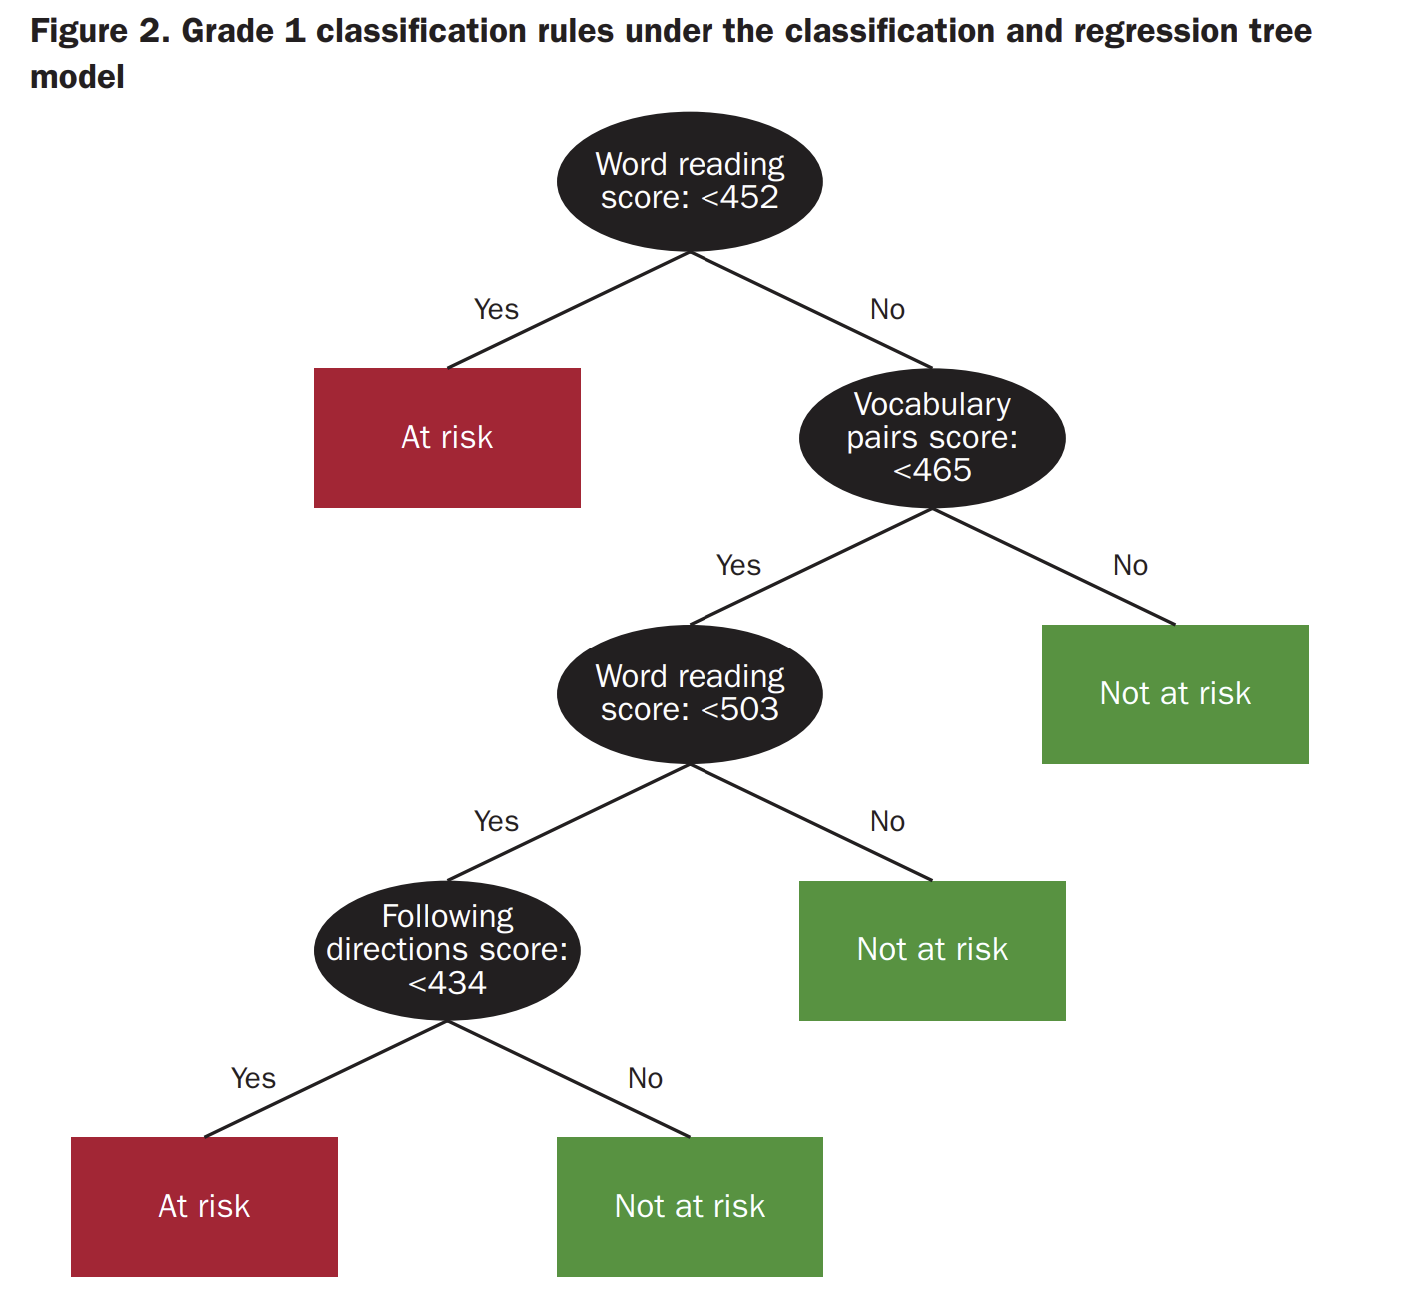
\includegraphics[width=\linewidth]{images/hall_decision_tree_example.png}

\vspace{0.2em}
\tiny\textit{Koon, Petscher \& Foorman (2014), REL Southeast. Reproduced from Hall (2025).}
\end{center}
\end{column}
\end{columns}
\end{frame}

\begin{frame}{The Problem with Single Trees}
\begin{columns}[T]
\begin{column}{0.55\textwidth}
\begin{itemize}
  \setlength\itemsep{0.4em}
  \item \textbf{High variance:} a small change in training data can produce a completely different tree
  \item \textbf{Overfitting:} a deep tree memorises the training data and performs poorly on new cases
  \item \textbf{Weak learner:} reasonable accuracy on its own, but far from state of the art
\end{itemize}

\vspace{0.7em}
\begin{alertblock}{Intuition}
Asking one person a yes/no question is unreliable.\\
Asking 500 people and taking a majority vote is much more robust.
\end{alertblock}
\end{column}
\begin{column}{0.42\textwidth}
\textbf{Overfitting vs.\ underfitting}
\vspace{0.5em}

\resizebox{\linewidth}{!}{%
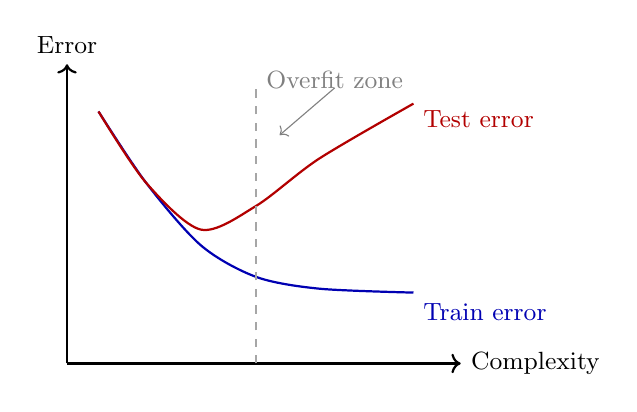
\begin{tikzpicture}[font=\small]
\draw[->, thick] (0,0) -- (5.0,0) node[right] {Complexity};
\draw[->, thick] (0,0) -- (0,3.8) node[above] {Error};

\draw[blue!70!black, thick, smooth]
  plot coordinates {(0.4,3.2)(1.0,2.3)(1.7,1.5)(2.4,1.1)(3.2,0.95)(4.4,0.90)};
\draw[red!70!black, thick, smooth]
  plot coordinates {(0.4,3.2)(1.0,2.3)(1.7,1.7)(2.4,2.0)(3.2,2.6)(4.4,3.3)};

\draw[dashed, gray!70] (2.4,0) -- (2.4,3.5);

\node[blue!70!black, right, font=\small] at (4.4,0.65) {Train error};
\node[red!70!black,  right, font=\small] at (4.4,3.10) {Test error};
\node[gray, font=\small] at (3.4,3.6) {Overfit zone};
\draw[->, gray, thin] (3.4,3.5) -- (2.7,2.9);
\end{tikzpicture}}
\end{column}
\end{columns}
\end{frame}

% =============================================================================
\section{Ensemble Methods}

\begin{frame}{Random Forests: Wisdom of the Crowd}
\begin{columns}[T]
\begin{column}{0.55\textwidth}
\textbf{How it works}
\begin{enumerate}
  \setlength\itemsep{0.35em}
  \item Draw a \textbf{bootstrap sample} of the training data (random rows, with replacement)
  \item Grow a full decision tree -- but at each split consider only a \textbf{random subset of features}
  \item Repeat for $N$ trees (typically 100--500)
  \item Final prediction: \textbf{majority vote} (classification) or \textbf{average} (regression)
\end{enumerate}

\vspace{0.6em}
\textbf{Why it works}
\begin{itemize}
  \item Each tree sees different data and different features
  \item Errors in individual trees are uncorrelated
  \item Averaging uncorrelated errors cancels them out
\end{itemize}
\end{column}
\begin{column}{0.42\textwidth}
\begin{block}{Out-of-bag (OOB) error}
Each bootstrap sample leaves out roughly 37\% of training rows. These unseen rows form a natural test set for that tree -- giving a free estimate of generalisation error without touching the held-out test set.
\end{block}

\vspace{0.6em}
\begin{block}{Variable importance}
For each feature: randomly permute its values and measure how much accuracy drops. A large drop means the feature is important for prediction.
\end{block}
\end{column}
\end{columns}
\end{frame}

\begin{frame}{Gradient Boosting: Learning from Mistakes}
\begin{columns}[T]
\begin{column}{0.55\textwidth}
\textbf{Key idea: sequential improvement}
\begin{enumerate}
  \setlength\itemsep{0.35em}
  \item Start with a simple initial prediction (e.g., the class majority)
  \item Fit a shallow tree to the \textbf{residuals} (errors) of the current model
  \item Add that tree to the ensemble, scaled by a \textbf{learning rate}
  \item Repeat for many iterations
\end{enumerate}

\vspace{0.5em}
\textbf{Difference from random forests}
\begin{itemize}
  \item RF: trees grow \textit{in parallel}, each independent
  \item GB: trees grow \textit{sequentially}, each correcting the previous
\end{itemize}
\end{column}
\begin{column}{0.42\textwidth}
\textbf{Key hyperparameters}
\vspace{0.4em}

\small
\renewcommand{\arraystretch}{1.3}
\begin{tabular}{ll}
\toprule
Parameter & Effect \\
\midrule
\texttt{n\_estimators}  & Number of trees \\
\texttt{learning\_rate} & Step size per tree \\
\texttt{max\_depth}     & Tree complexity \\
\texttt{subsample}      & Row sampling fraction \\
\bottomrule
\end{tabular}

\vspace{0.8em}
\begin{alertblock}{Overfitting risk}
Gradient boosting can overfit if too many trees are grown. Monitor training vs.\ test error as iterations increase.
\end{alertblock}
\end{column}
\end{columns}
\end{frame}

\begin{frame}{Comparing the Three Methods}

\begin{center}
\small
\renewcommand{\arraystretch}{1.4}
\begin{tabular}{lccc}
\toprule
 & \textbf{Decision Tree} & \textbf{Random Forest} & \textbf{Gradient Boosting} \\
\midrule
Training speed     & Fast     & Moderate & Slow \\
Predictive accuracy & Moderate & High     & Very high \\
Interpretability   & High     & Low      & Low \\
Overfitting risk   & High     & Low      & Moderate \\
Tuning required    & Minimal  & Some     & Significant \\
\bottomrule
\end{tabular}
\end{center}

\vspace{1em}
\begin{alertblock}{Practical advice for social scientists}
Start with a random forest. It is robust, requires minimal tuning, and gives you variable importance for free. Move to gradient boosting if you need the last increment of accuracy and have time to tune carefully.
\end{alertblock}
\end{frame}

% =============================================================================
\section{Model Evaluation}

\begin{frame}{Evaluating Model Performance: The Confusion Matrix}
\begin{columns}[T]
\begin{column}{0.52\textwidth}
\vspace{0.2em}
\small
\renewcommand{\arraystretch}{1.35}
\begin{tabular}{l|cc}
 & \textbf{Pred.\ $>$\$50K} & \textbf{Pred.\ $\leq$\$50K} \\
\hline
\textbf{Actual $>$\$50K} & \cellcolor{green!15}True Positive (TP) & \cellcolor{red!12}False Negative (FN) \\
\textbf{Actual $\leq$\$50K} & \cellcolor{red!12}False Positive (FP) & \cellcolor{green!15}True Negative (TN) \\
\end{tabular}

\vspace{0.7em}
\small
\textbf{Accuracy} $= \dfrac{TP + TN}{N}$ \hfill \textit{misleading if imbalanced}

\vspace{0.35em}
\textbf{Precision} $= \dfrac{TP}{TP + FP}$ \hfill \textit{quality of positive predictions}

\vspace{0.35em}
\textbf{Recall} $= \dfrac{TP}{TP + FN}$ \hfill \textit{coverage of positives}

\vspace{0.35em}
\textbf{F1} $= 2 \cdot \dfrac{P \times R}{P + R}$ \hfill \textit{harmonic mean of P and R}
\end{column}

\begin{column}{0.45\textwidth}
\textbf{In our dataset (25\% earn $>$\$50K):}
\begin{itemize}
  \setlength\itemsep{0.3em}
  \item A ``predict everyone $\leq$\$50K'' model gets \textbf{75\% accuracy} but 0\% recall for the minority class
  \item Our models score $\approx$\textbf{84--87\% accuracy} -- but always report recall and F1 too
  \item Published benchmarks for this dataset: 85--87\% (Kohavi, 1996)
\end{itemize}

\vspace{0.4em}
\begin{alertblock}{When to use which metric}
\textbf{Precision:} when false alarms are costly (e.g., wrongly flagging someone)\\
\textbf{Recall:} when missing a case is costly (e.g., missing a disease)\\
\textbf{F1:} when both matter equally
\end{alertblock}
\end{column}
\end{columns}
\end{frame}

% =============================================================================
\section{Unsupervised Learning: Clustering}

\begin{frame}{Finding Hidden Groups in Your Data}
\begin{columns}[T]
\begin{column}{0.55\textwidth}
\textbf{What clustering does}
\begin{itemize}
  \setlength\itemsep{0.35em}
  \item No outcome variable: we look for natural groupings in the data
  \item Groups observations that are similar to each other and dissimilar from other groups
  \item Output: a cluster label for each observation, plus characterisation of each group
\end{itemize}

\vspace{0.5em}
\textbf{K-means algorithm}
\begin{enumerate}
  \setlength\itemsep{0.3em}
  \item Choose $k$ (number of clusters)
  \item Assign $k$ random centroids
  \item Assign each observation to its nearest centroid
  \item Recalculate centroids as the mean of each cluster
  \item Repeat steps 3--4 until stable
\end{enumerate}
\end{column}
\begin{column}{0.42\textwidth}
\textbf{Social science applications}
\vspace{0.4em}
\begin{itemize}
  \setlength\itemsep{0.35em}
  \item \textbf{Typology building:} replace subjective manual classification with a data-driven partition
  \item \textbf{Survey analysis:} identify latent respondent profiles
  \item \textbf{Policy targeting:} segment populations for differentiated intervention
  \item \textbf{Exploratory research:} discover structure when you have no prior hypothesis
\end{itemize}

\vspace{0.5em}
\begin{alertblock}{Choosing $k$}
Plot within-cluster variance against $k$. Look for the \textit{elbow}: the point where adding more clusters stops making a large difference.
\end{alertblock}
\end{column}
\end{columns}
\end{frame}

% =============================================================================
\section{What ML Cannot Do}

\begin{frame}{Limits and Ethical Considerations}
\begin{columns}[T]
\begin{column}{0.48\textwidth}
\textbf{Conceptual limits}
\begin{itemize}
  \setlength\itemsep{0.4em}
  \item \textbf{Correlation is not causation:} ML finds patterns, not mechanisms. A model that predicts poverty accurately does not tell you what causes it.
  \item \textbf{Garbage in, garbage out:} model quality depends entirely on data quality and representativeness
  \item \textbf{Black box problem:} complex models are difficult to explain to a reviewer, a judge, or a policymaker
\end{itemize}
\end{column}
\begin{column}{0.48\textwidth}
\textbf{Ethical risks}
\begin{itemize}
  \setlength\itemsep{0.4em}
  \item \textbf{Encoded bias:} if training data reflects historical inequality, the model will reproduce and amplify it
  \item \textbf{Differential accuracy:} models often perform worse for minority or underrepresented groups
  \item \textbf{Feedback loops:} predictions inform decisions that generate new data, reinforcing the original pattern
\end{itemize}
\end{column}
\end{columns}

\vspace{0.9em}
\begin{center}
\alert{ML is a tool, not an oracle. The researcher's theoretical and ethical judgement remains indispensable.}
\end{center}
\end{frame}

% =============================================================================
\section{Today's Practical}

\begin{frame}{Practical Overview: 1994 US Census Income Data}
\begin{columns}[T]
\begin{column}{0.55\textwidth}
\textbf{The dataset}
\begin{itemize}
  \setlength\itemsep{0.35em}
  \item 48,842 adults from the 1994 US Census
  \item \textbf{Task:} predict income $>$\$50K or $\leq$\$50K
  \item \textbf{Features:} age, education level, occupation, marital status, sex, race, hours worked per week, country of origin
  \item Directly relevant to questions of labour market inequality, demographic disparities, and social stratification
\end{itemize}

\vspace{0.5em}
\textbf{What we will build}
\begin{enumerate}
  \item Decision tree classifier
  \item Random forest classifier
  \item Gradient boosting classifier
  \item[] \textit{Extension:} K-means clustering
\end{enumerate}
\end{column}
\begin{column}{0.42\textwidth}
\textbf{How to access}
\vspace{0.4em}

\begin{enumerate}
  \setlength\itemsep{0.4em}
  \item Open:\\
        \small\texttt{github.com/BHannan01/}\\
        \texttt{introduction-to-machine-learning}
  \item Click \textbf{Open in Colab}\\
        on the notebook file
  \item The notebook downloads data automatically
  \item Run cells top to bottom
\end{enumerate}

\vspace{0.8em}
\begin{alertblock}{No installation needed}
Google Colab runs entirely in your browser. You only need a Google account.
\end{alertblock}

\vspace{0.4em}
\small\textit{All code is heavily commented. Reflection questions appear throughout.}
\end{column}
\end{columns}
\end{frame}

% ─── Closing ─────────────────────────────────────────────────────────────────
\begin{frame}[standout]
\Large Questions?

\vspace{1.2em}
\normalsize
\texttt{github.com/BHannan01/introduction-to-machine-learning}\\[0.4em]
\texttt{brody.hannan@soton.ac.uk}
\end{frame}

\end{document}
